\section{Classification of states}
\begin{definition}[]
    We say that state $j$ is \textit{accessible} from state $i$, written as $ i \to j $, If  $ p^{n}_{ij}>0 $ for some $ n\ge 0 $.\\ 
    We assume every state is accessible from itself since
    \[
        p^{0}_{ii} = \mathbf{P}(X_{0}=i|X_{0}=i) = 1.
    \]
\end{definition}

\begin{definition}[]
    Two states $i$ and $j$ are said to \textit{communicate} , written as $ i \longleftrightarrow j $, if they are accessible from each other.\\ 
    i.e.
    \[
        i\longleftrightarrow j \implies i \to j \ \And j\to i
    \]
\end{definition}

Communication is an equivalence relation. That means that,
\begin{enumerate}
    \item $ i\longleftrightarrow i $,
    \item if $ i\longleftrightarrow j $ then  $ j\longleftrightarrow i$,
    \item if  $ i\longleftrightarrow j $ and  $ j\longleftrightarrow k $ then  $ i\longleftrightarrow k $.
\end{enumerate}

First two properties are obvious from definition, let for some $n,\ m \ge 0$ then, $ p^{n}_{ij},\ p^{m}_{jk}>0 $ by assumption.
By Chapman-Kolmogorov equatation.
\[
    p^{n+m}_{ik} = \sum_{r=0}^{\infty} p^{n}_{ir}p^{m}_{rk} \ge p^{n}_{ij}p^{m}_{jk}>0.
\]
Hence state k is accessible from state i. By same one can prove that $i$ is also accessible from $K$.

Therefore, the states of a Markov chain can be partitioned into communicating classes such that 
only members of the same class communicate with each other. 
i.e. two states $ i \ \&\ j $ belong to same class if and only if $ i\longleftrightarrow j $.

\begin{example}[]
    Consider the markov chain define in the picture \cref{example of communication}.
\begin{figure}[h]
    \centering
    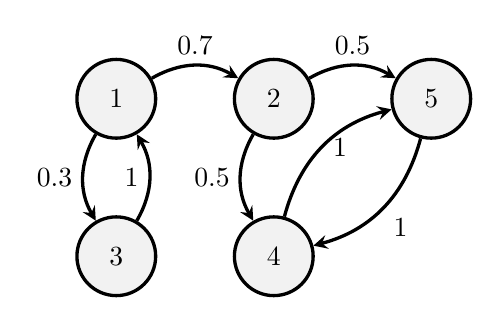
\begin{tikzpicture}[->, >=stealth, auto, very thick, node distance = 2cm, state/.style={circle, draw=black, fill=black!5, very thick, minimum size = 10mm}]
        \node[state] (1) {$1$};
        \node[state] (2) [right of=1] {$2$};
        \node[state] (3) [below of=1] {$3$};
        \node[state] (4) [below of=2] {$4$};
        \node[state] (5) [right of=2] {$5$};

        \path (1) edge [bend right] node [left] {0.3} (3)
              (1) edge [bend left] node [above] {0.7} (2)
              (3) edge [bend right] node {1} (1)
              (2) edge [bend right] node [left] {0.5} (4)
              (2) edge [bend left] node {0.5} (5)
              (4) edge [bend left] node [right] {1} (5)
              (5) edge [bend left] node {1} (4);
    \end{tikzpicture}
    \caption{Communication classes}
    \label{example of communication}
\end{figure}

here the classes are $\{ 1,3 \}, \{2\}, \{4,5\}$
\end{example}

\begin{definition}[Irreducible Markov chain]
    A Markov chain is said to be irreducible if it has only one communicating class. That is, every state communicate with each other.\\ 
    That is, for any states $i$, $j$ there is some positive integer $n$ such that the $(i, j)$ entry of $ P^{n} $ is positive.
\end{definition}

A Markov chain that is not irreducible called reducible.

For any state $ i $ and $ j $ define $ f^{n}_{ij} $ to be the probability that, starting from $ i $, the first transition into $ j  $
occurs at $ n $ time. \\ 
i.e. 
\[
    f^{n}_{ij} = \mathbf{P}(X_{n},X_{k}\neq j, k=1,2,\ldots n-1|X_{0}=i).
\]
Let
\[
    f^*_{ij}=\sum_{n=0}^{\infty} f^{n}_{ij}
\]

Then, $ f^*_{ij} $ denote the probability of ever making a transition into step $ j $ when start from state $ i $. 
If $ j $ is not accessible from $ i $ then $ f^*_{ij} $ will be zero.

\begin{definition}[Recurrent and Transient state]
    A state $ j $ of a Markov chain is said to be \textit{recurrent}  $ f^*_{ii}=1 $ and \textit{transient}  if $ f^*_{ii}<1 $.
\end{definition}

In other word, if a Markov chain start in a recurrent state, there is a guarantee that it will visit that state again in the future
(eventually return to that state with probability 1).

In contrast, a transient state in a Markov chain is a state where, once you reach it, 
there is a positive probability that you will never return to that state.
i.e. if you begin in a transient state, there's a chance you won't return there.

\begin{corollary}
    \label{recurrent}
    state $ i $ is recurrent if and only if  $ \sum_{n=0}^{\infty} p^{n}_{ii}=\infty $
\end{corollary}
\begin{proof}
    The state $ i $ is recurrent if and only if, starting in state  $ i $, the expected number of time periods that the 
    process is in state  $ i $ is infinite. \\ 
    Let
    \[
        I_{n} =
        \begin{cases}
            1, \ \ &\text{if}\ X_{n} = i\\ 
            0, \ \ &\text{if}\ X_{n} \neq  i\\ 
        \end{cases}
    \]
    we then have $ \sum_{n=0}^{\infty} I_{n} $ represent the number of periods that the process is in state $ i $ Then,

    \begin{align*}
        E\left[\sum_{n=0}^{\infty} I_{n}|X_{0}=i\right]&= \sum_{n=0}^{\infty} E[I_{n}|X_{0}=i] \\
        &= \sum_{n=0}^{\infty} \mathbf{P}(X_{n}=i|X_{0}=i) \\
        &= \sum_{n=0}^{\infty} p^{n}_{ii} 
    \end{align*}
    Hence the result.
\end{proof}

\begin{theorem}[]
    \label{recurent if communicate}
    If $ i $ is recurrent and $ i\longleftrightarrow j $, then  $ j $ is also recurrent.
\end{theorem}
\begin{proof}
    Let $ m $ and  $ k $ be such that  $ p^{k}_{ij}>0,p^{m}_{ji}>0 $. Now for any $ n\ge 0 $
    \[
        p^{m+n+k}_{jj}\ge p^{m}_{ji}p^{k}_{ii}p^{m}_{ij}
    \]
    This follows because the left-hand side of the preceding equation is the probability of going $j \to j$ in $m+n+k$ steps,
      whereas the right-hand side is the probability of going $j \to j$ in $m+n+k$ steps
      via a path that goes from $j \to i$ in $m$ steps, then $i \to i$ in $n$ additional steps,
      then $i \to $j in $k$ additional steps. By summing the preceding over n. we obtain
    \[
        \sum_{n=0}^{\infty} p^{m+n+k}_{jj}\ge p^{m}_{ji}p^{k}_{ii} \sum_{n=0}^{\infty}  p^{n}_{ij} = \infty
    \]
     where $ \sum_{n=0}^{\infty}  p^{n}_{ij} = \infty $ because state $ i $ is recurrent. Thus, $j$ is also recurrent.
\end{proof}

\begin{proposition}
     In an irreducible Markov chain with a finite state space, all states are recurrent.
\end{proposition}

\begin{definition}[Absorbing State]
    A state $ i $ of Markov chain is called absorbing it  $ p_{ii} = 1 $ that is, it is impossible to leave 
    the state. 
\end{definition}

A Markov Chain is absorbing if it has at least one absorbing state.

For example consider the Markov chain shown in Fig. \ref{Absorving markov chain}

\begin{figure}[H]
    \centering
    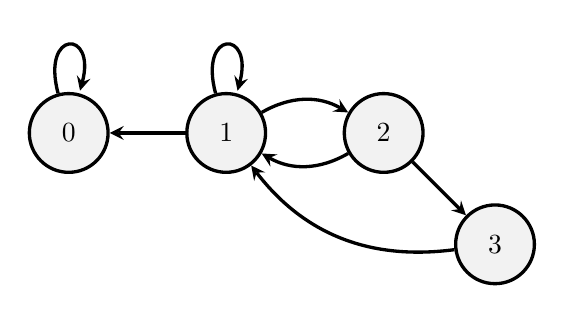
\begin{tikzpicture}[->, >=stealth, auto, very thick, node distance = 2cm, state/.style={circle, draw=black, fill=black!5, very thick, minimum size = 10mm}]
        \node[state] (0) {0};
        \node[state] (1) [right of=0] {1};
        \node[state] (2) [right of=1] {2};
        \node[state] (3) [below right of=2] {3};

        \path (0) edge [loop above] (0)
        (1) edge [] (0)
        (1) edge [loop above] (1)
        (1) edge [bend left] (2)
        (2) edge [bend left] (1)
        (2) edge [] (3)
        (3) edge [bend left] (1);
    \end{tikzpicture}
    \centering
    \caption{Absorbing Markov Chain}
    \label{Absorving markov chain}
\end{figure}

here $p_00=1$ hence, State 0 is Absorbing State in this case.
